\section{MÔ HÌNH MẠNG CAMPUS ĐỀ XUẤT}\label{sec:mo_hinh_de_xuat}

Chương này trình bày thiết kế của hệ thống mạng Campus đa cơ sở: phân tích yêu cầu, kiến trúc tổng thể, topology chi tiết từng site, quy hoạch VLAN và địa chỉ IP, thiết kế định tuyến, thiết kế SDN, thiết kế SD-WAN, thiết kế dịch vụ và chính sách bảo mật. Mọi thông số trong chương đều thống nhất với cấu hình đang vận hành của các thiết bị trong mô hình.

\subsection{Phân tích bài toán và yêu cầu thiết kế}

\subsubsection{Bối cảnh bài toán}

Đề tài giả định một trường đại học có một cơ sở chính và ba cơ sở phụ đặt tại Cần Thơ, Đà Nẵng và Nha Trang. Cơ sở chính tập trung các khoa Công nghệ thông tin, Toán -- Thống kê, Luật, khối Hành chính, cùng toàn bộ dịch vụ dùng chung (DHCP, DNS, Web, Mail, Syslog). Mỗi cơ sở phụ có hai khối nghiệp vụ riêng và cần truy cập các dịch vụ dùng chung tại cơ sở chính.

Trong mô hình mạng truyền thống, mỗi switch tự học địa chỉ, tự chạy STP và được cấu hình thủ công; kết nối giữa các cơ sở thường dựa vào một đường truyền riêng với cấu hình định tuyến tĩnh tại từng router. Khi số VLAN, số thiết bị và số cơ sở tăng lên, cách quản trị này bộc lộ ba vấn đề: (1) thay đổi chính sách phải thực hiện trên nhiều thiết bị, dễ sai lệch; (2) không có cái nhìn toàn cục về trạng thái lớp 2 và lưu lượng; (3) kết nối WAN phụ thuộc một đường truyền, không tự chọn đường theo chất lượng.

Bài toán đặt ra là xây dựng một mạng Campus đa cơ sở trong đó: mạng nội bộ cơ sở chính được điều khiển tập trung bằng SDN Controller; các cơ sở được kết nối qua overlay SD-WAN chạy trên hai nhà cung cấp độc lập (Internet và MPLS), có lựa chọn đường theo SLA và chính sách tập trung; đồng thời vẫn giữ các cơ chế truyền thống đã được kiểm chứng (VRRP, OSPF, tường lửa HA) tại những vị trí cần độ ổn định cao.

\subsubsection{Yêu cầu chức năng}

\begin{itemize}
    \item \textbf{Kết nối:} máy trạm tại mọi cơ sở truy cập được dịch vụ dùng chung ở cơ sở chính; các cơ sở phụ liên lạc được với nhau khi chính sách cho phép.
    \item \textbf{Phân đoạn:} mỗi khoa/khối nghiệp vụ là một VLAN và một subnet riêng; vùng máy chủ, vùng DMZ và vùng quản trị được tách biệt.
    \item \textbf{Cấp phát địa chỉ:} máy trạm nhận địa chỉ động qua DHCP; máy chủ và thiết bị hạ tầng dùng địa chỉ tĩnh.
    \item \textbf{Dịch vụ:} DNS nội bộ cho tên miền \texttt{campus.internal}, Web (HTTPS), Mail (SMTP/IMAP) và Syslog tập trung.
    \item \textbf{Điều khiển SDN:} Controller quản lý toàn bộ chuyển mạch lớp 2 tại tầng Distribution và Access của cơ sở chính, chống vòng lặp, hỗ trợ chặn cổng tập trung, cung cấp REST API và giám sát tải cổng.
    \item \textbf{SD-WAN:} các Edge được xác thực bằng chứng thư, hình thành overlay IPsec trên hai transport, phân phối tuyến qua OMP, áp chính sách SLA/AAR và lọc lưu lượng tập trung.
    \item \textbf{Bảo mật biên:} tường lửa kiểm soát lưu lượng giữa nội bộ, DMZ và WAN theo nguyên tắc chỉ mở dịch vụ cần thiết.
\end{itemize}

\subsubsection{Yêu cầu phi chức năng}

\begin{itemize}
    \item \textbf{Tính sẵn sàng:} không có điểm lỗi đơn tại gateway (VRRP), lõi (hai Core, EtherChannel), biên (tường lửa Active/Standby), WAN (hai Edge, hai transport) và lớp 2 (Access nối kép lên hai Distribution).
    \item \textbf{Khả năng mở rộng:} quy tắc địa chỉ thống nhất theo site; một cơ sở mới chỉ cần cấp Site-ID, System-IP, subnet và dùng lại khuôn cấu hình chi nhánh.
    \item \textbf{Khả năng quản trị:} vùng quản trị riêng, giao diện quản trị tập trung (ASDM, vManage, REST/GUI của SDN Controller), nhật ký tập trung.
    \item \textbf{Tính nhất quán:} mỗi thiết bị có định danh, địa chỉ và vai trò rõ ràng, được ghi nhận trong các bảng quy hoạch.
\end{itemize}

\subsubsection{Phạm vi và giả định}

Hệ thống được hiện thực trên nền tảng mô phỏng EVE-NG bằng các image thiết bị thương mại và mã nguồn mở. Hai nhà cung cấp dịch vụ được mô phỏng bằng hai router chạy BGP; mạng Internet công cộng được mô phỏng bằng dải địa chỉ tài liệu \texttt{203.0.113.0/24}, còn mạng MPLS dùng dải \texttt{100.64.0.0/10}. Mạng không dây, xác thực 802.1X và kết nối Internet thật của người dùng nằm ngoài phạm vi triển khai và được nêu ở phần hướng phát triển.

\subsection{Kiến trúc tổng thể}

Hệ thống gồm năm khối chức năng và hai miền truyền tải, được tổng hợp trong Bảng~\ref{tab:cac_site}.

\begin{table}[H]
    \centering
    \small
    \caption{Các site và vai trò trong mô hình}
    \label{tab:cac_site}
    \begin{tabularx}{\textwidth}{|c|P{2.6cm}|c|X|}
        \hline
        \textbf{Site-ID} & \textbf{Tên} & \textbf{ASN} & \textbf{Thành phần chính} \\
        \hline
        100 & Campus chính & 65000 & Cặp tường lửa ASAv HA, Core-SW1/2, Dist-SW1/2 và Access-SW1--4 (Open vSwitch), SDN Controller (Ryu, ONOS), Server Farm, DMZ, hai vEdge \\
        \hline
        200 & Cơ sở Cần Thơ & 65010 & Brand-FW, SwitchBrand, hai switch khối, hai vEdge; VLAN 60 Nông nghiệp, 70 Y tế \\
        \hline
        300 & Cơ sở Đà Nẵng & 65020 & Cấu trúc như Site 200; VLAN 80 Du lịch, 90 Tài chính \\
        \hline
        400 & Cơ sở Nha Trang & 65030 & Cấu trúc như Site 200; VLAN 50 Thủy sản, 60 Lữ hành \\
        \hline
        900 & Trung tâm điều khiển SD-WAN & -- & vManage, vSmart, vBond, Switch32 (LAN controller), Switch61 (mặt quản trị), máy trạm quản trị, vEdge65 dự phòng \\
        \hline
        -- & Nhà cung cấp Internet & 64511 & Router Internet, color \texttt{biz-internet} \\
        \hline
        -- & Nhà cung cấp MPLS & 64512 & Router MPLS, color \texttt{mpls} \\
        \hline
    \end{tabularx}
\end{table}

Kiến trúc được tổ chức theo ba mặt phẳng:
\begin{itemize}
    \item \textbf{Mặt phẳng dữ liệu} gồm các switch, tường lửa, Edge và router nhà cung cấp, chuyển tiếp lưu lượng người dùng.
    \item \textbf{Mặt phẳng điều khiển} gồm hai miền độc lập: SDN Controller điều khiển lớp 2 cơ sở chính qua OpenFlow 1.3 trên VLAN 99; vSmart điều khiển overlay SD-WAN qua OMP. Tại lớp 3 cơ sở chính, OSPF và VRRP vẫn là cơ chế điều khiển phân tán.
    \item \textbf{Mặt phẳng quản trị} gồm VLAN 99 tại cơ sở chính (ASDM, REST/GUI của Controller, giám sát) và mạng \texttt{10.9.0.0/24}, \texttt{10.9.1.0/24} tại Site 900 (vManage).
\end{itemize}

Nguyên tắc phân vai quan trọng là \textit{mỗi thành phần chỉ làm đúng việc của mình}: Core Switch chỉ định tuyến liên VLAN và làm gateway; OVS chỉ chuyển mạch lớp 2 theo flow của Controller; tường lửa kiểm soát biên và DMZ; vEdge chỉ làm router WAN và đầu cuối overlay; tường lửa chi nhánh kiêm gateway và DHCP cho chi nhánh. Hình~\ref{fig:topology_mang_campus} trình bày topology logic ở mức site.

\begin{figure}[H]
    \centering
    \resizebox{\textwidth}{!}{%
    \begin{tikzpicture}[
        font=\scriptsize,
        >=stealth,
        controller/.style={draw=purple!70!black, fill=purple!7, rounded corners, align=center, minimum height=1.35cm, text width=8.0cm},
        transport/.style={draw=black!70, fill=gray!12, rounded corners, align=center, minimum height=0.9cm, text width=3.5cm},
        campus/.style={draw=blue!65!black, fill=blue!5, rounded corners, align=center, minimum height=1.75cm, text width=6.2cm},
        branch/.style={draw=teal!70!black, fill=teal!5, rounded corners, align=center, minimum height=1.55cm, text width=5.1cm},
        controlLink/.style={draw=purple!75!black, dashed, ->, line width=0.7pt},
        internetLink/.style={draw=blue!75!black, line width=0.9pt},
        mplsLink/.style={draw=orange!85!black, line width=0.9pt}
    ]
        \node[controller] (s900) at (0,5.1) {\textbf{Site 900 -- Mặt phẳng điều khiển SD-WAN}\\
        vManage \texttt{10.9.0.10}; vSmart \texttt{10.9.0.11} (System-IP \texttt{10.9.0.13}); vBond \texttt{10.9.0.12}\\
        Switch32 gateway \texttt{10.9.0.2}; vEdge65 dự phòng (System-IP \texttt{10.200.90.1})};

        \node[transport] (internet) at (-4.6,3.25) {\textbf{Internet underlay}\\AS 64511 -- color \texttt{biz-internet}};
        \node[transport] (mpls) at (4.6,3.25) {\textbf{MPLS underlay}\\AS 64512 -- color \texttt{mpls}};

        \node[campus] (s100) at (0,1.35) {\textbf{Site 100 -- Campus chính, AS 65000}\\
        vEdge1/2: \texttt{10.200.100.1/.2}, mỗi Edge có TLOC Internet và MPLS\\
        ASAv HA -- Core-SW1/2 -- Ryu \texttt{10.1.99.10} điều khiển 6 OVS -- VLAN 10/20/30/40/90/99};

        \node[branch] (s200) at (-6.1,-1.35) {\textbf{Site 200 -- Cần Thơ, AS 65010}\\
        vEdge1 \texttt{10.200.200.1} (MPLS)\\vEdge2 \texttt{10.200.200.2} (Internet)\\Brand-FW -- VLAN 60/70};
        \node[branch] (s300) at (0,-1.35) {\textbf{Site 300 -- Đà Nẵng, AS 65020}\\
        vEdge1 \texttt{10.200.30.1} (MPLS)\\vEdge2 \texttt{10.200.30.2} (Internet)\\Brand-FW -- VLAN 80/90};
        \node[branch] (s400) at (6.1,-1.35) {\textbf{Site 400 -- Nha Trang, AS 65030}\\
        vEdge1 \texttt{10.200.40.1} (MPLS)\\vEdge2 \texttt{10.200.40.2} (Internet)\\Brand-FW -- VLAN 50/60};

        \begin{pgfonlayer}{background}
            \draw[internetLink] (internet) -- (s100.north west);
            \draw[internetLink] (internet.south) -- (s200.north);
            \draw[internetLink] (internet.south east) -- (s300.north west);
            \draw[internetLink] (internet.east) -- (s400.north west);
            \draw[mplsLink] (mpls) -- (s100.north east);
            \draw[mplsLink] (mpls.west) -- (s200.north east);
            \draw[mplsLink] (mpls.south west) -- (s300.north east);
            \draw[mplsLink] (mpls.south) -- (s400.north);
            \draw[internetLink] (internet) -- (s900.south west);
            \draw[mplsLink] (mpls) -- (s900.south east);

            \draw[controlLink] (s900.south) -- (s100.north);
            \draw[controlLink] (s900.south west) to[bend right=18] (s200.north);
            \draw[controlLink] (s900.south) to[bend right=10] (s300.north);
            \draw[controlLink] (s900.south east) to[bend left=18] (s400.north);
        \end{pgfonlayer}

        \node[align=center, font=\scriptsize] at (0,-3.0) {\textcolor{blue!75!black}{\rule{1.0cm}{0.8pt}} Internet \quad
        \textcolor{orange!85!black}{\rule{1.0cm}{0.8pt}} MPLS \quad
        \textcolor{purple!75!black}{- - - $\triangleright$} Kết nối điều khiển DTLS/OMP};
    \end{tikzpicture}%
    }
    \caption{Topology logic của hệ thống ở mức site}
    \label{fig:topology_mang_campus}
\end{figure}

Hình~\ref{fig:kien_truc_tong_the_campus} là topology vật lý đầy đủ của hệ thống trên EVE-NG, gồm 67 node và 100 phân đoạn mạng. Các thông số địa chỉ chuẩn của từng thiết bị được trình bày trong các bảng quy hoạch ở Mục~\ref{sec:quy_hoach_ip}.

\begin{figure}[H]
    \centering
    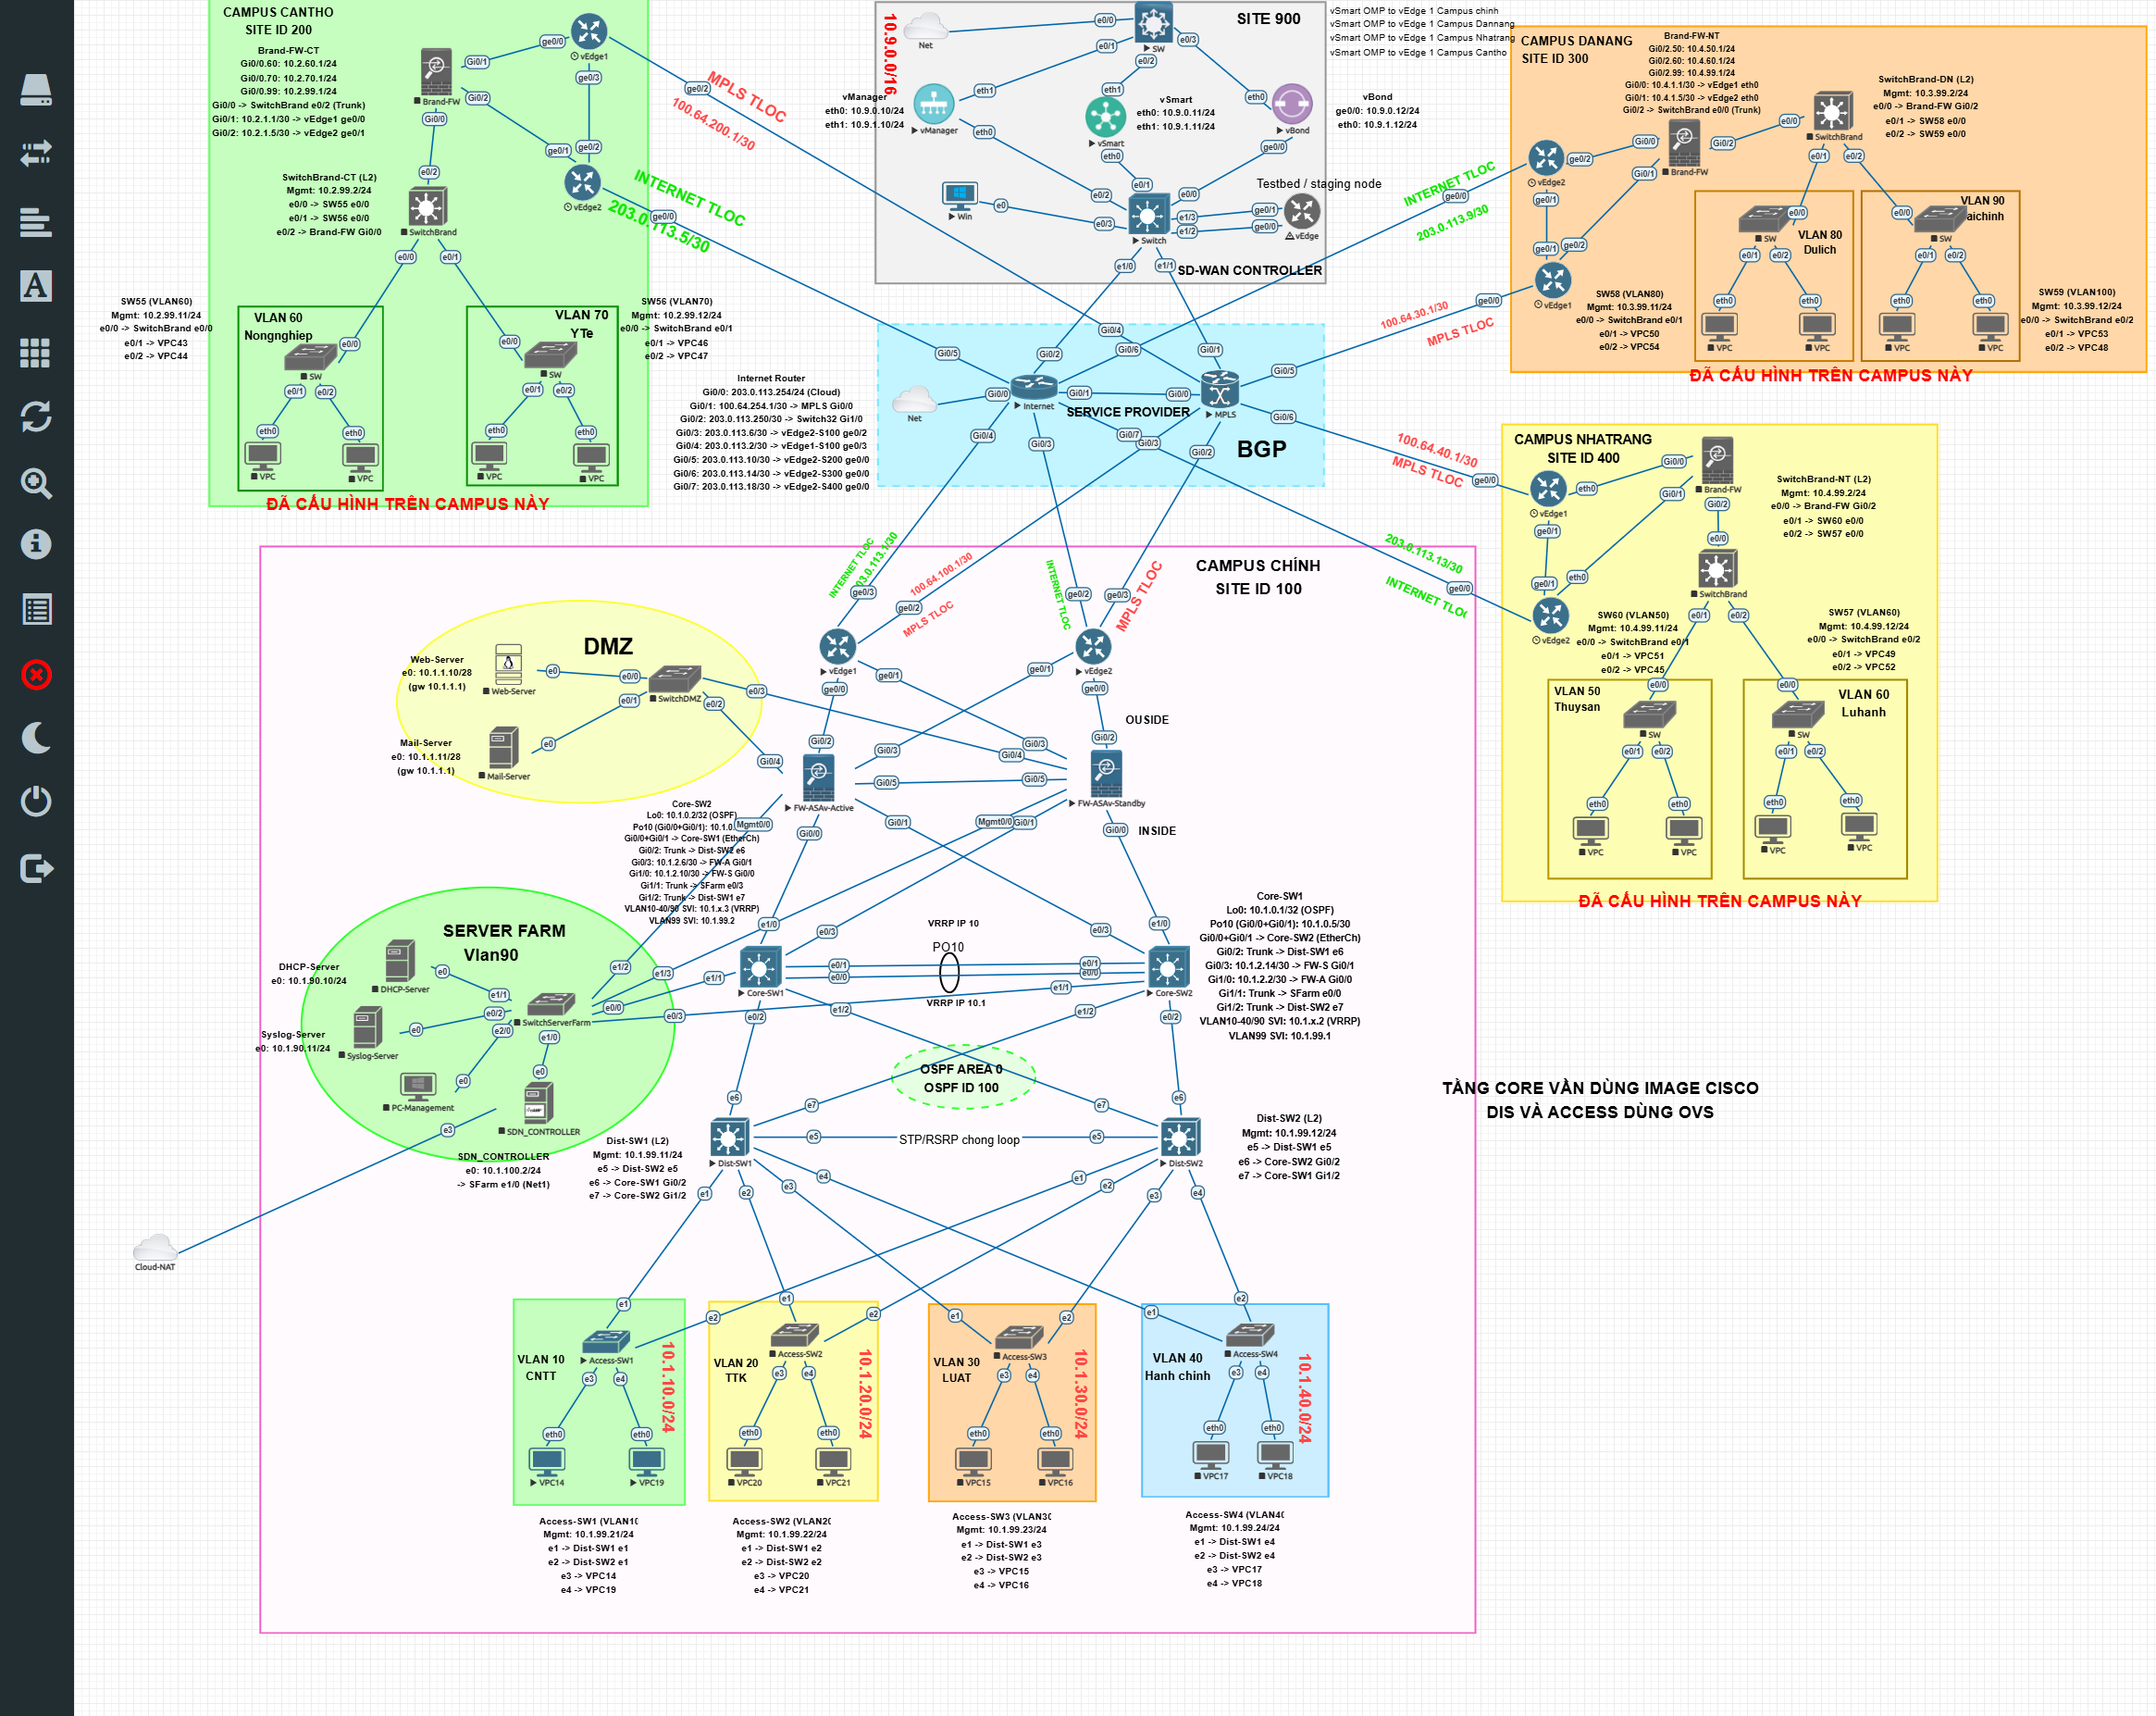
\includegraphics[width=\textwidth]{image/eve_topology.png}
    \caption{Topology vật lý của hệ thống trên EVE-NG}
    \label{fig:kien_truc_tong_the_campus}
\end{figure}

\subsection{Thiết kế topology chi tiết}

\subsubsection{Campus chính (Site 100)}

Campus chính được thiết kế ba tầng, kèm biên tường lửa HA, vùng DMZ và vùng Server Farm như Hình~\ref{fig:topology_site100}.

\begin{figure}[H]
    \centering
    \resizebox{\textwidth}{!}{%
    \begin{tikzpicture}[
        font=\scriptsize, >=stealth,
        dev/.style={draw, rounded corners, align=center, minimum height=0.85cm, text width=2.5cm},
        wan/.style={dev, fill=gray!12, draw=black!60},
        edge/.style={dev, fill=red!6, draw=red!60!black},
        fw/.style={dev, fill=orange!10, draw=orange!70!black},
        core/.style={dev, fill=blue!8, draw=blue!65!black},
        ovs/.style={dev, fill=green!8, draw=green!45!black},
        srv/.style={dev, fill=yellow!10, draw=yellow!50!black, text width=3.6cm},
        act/.style={line width=0.9pt},
        stb/.style={dashed, line width=0.6pt}
    ]
        \node[wan] (inet) at (-2.2,9.2) {Internet\\AS 64511};
        \node[wan] (mpls) at (2.2,9.2) {MPLS\\AS 64512};
        \node[edge] (ve1) at (-2.2,7.6) {vEdge1-S100\\10.200.100.1};
        \node[edge] (ve2) at (2.2,7.6) {vEdge2-S100\\10.200.100.2};
        \node[fw] (fwa) at (-2.2,5.8) {FW-ASAv-Active\\Primary};
        \node[fw] (fws) at (2.2,5.8) {FW-ASAv-Standby\\Secondary};
        \node[srv] (dmz) at (-6.8,5.8) {DMZ 10.1.1.0/28\\SwitchDMZ (VLAN 101)\\Web .10 -- Mail .11};
        \node[core] (c1) at (-2.2,3.8) {Core-SW1\\VRRP Master};
        \node[core] (c2) at (2.2,3.8) {Core-SW2\\VRRP Backup};
        \node[srv] (farm) at (6.9,2.9) {SwitchServerFarm\\VLAN 90: DHCP/DNS .10, Syslog .11\\VLAN 99: Controller .10, PC-Mgmt .50, ASDM .33/.34};
        \node[ovs] (d1) at (-2.2,1.9) {Dist-SW1 (OVS)\\DPID 0x05};
        \node[ovs] (d2) at (2.2,1.9) {Dist-SW2 (OVS)\\DPID 0x08};
        \node[ovs] (a1) at (-5.4,0) {Access-SW1\\VLAN 10 CNTT};
        \node[ovs] (a2) at (-1.8,0) {Access-SW2\\VLAN 20 Toán-TK};
        \node[ovs] (a3) at (1.8,0) {Access-SW3\\VLAN 30 Luật};
        \node[ovs] (a4) at (5.4,0) {Access-SW4\\VLAN 40 Hành chính};

        \draw[act] (inet) -- (ve1); \draw[act] (inet) -- (ve2);
        \draw[act] (mpls) -- (ve1); \draw[act] (mpls) -- (ve2);
        \draw[act] (ve1) -- (fwa); \draw[act] (ve2) -- (fwa);
        \draw[stb] (ve1) -- (fws); \draw[stb] (ve2) -- (fws);
        \draw[act, orange!70!black] (fwa) -- node[above]{failover Gi0/5} (fws);
        \draw[act] (dmz) -- (fwa); \draw[stb] (dmz.south east) -- (fws);
        \draw[act] (fwa) -- (c1); \draw[act] (fwa) -- (c2);
        \draw[stb] (fws) -- (c1); \draw[stb] (fws) -- (c2);
        \draw[act, blue!65!black] (c1) -- node[above]{Po10} node[below]{LACP} (c2);
        \draw[act] ($(c1.south)+(0.9,0)$) |- (farm.west); \draw[stb] (c2.east) -- (farm.north west);
        \draw[act] (c1) -- (d1); \draw[stb] (c2) -- (d1);
        \draw[act] (c2) -- (d2); \draw[stb] (c1) -- (d2);
        \draw[stb] (d1) -- node[above]{inter-dist} (d2);
        \foreach \a in {a1,a2,a3,a4} {\draw[act] (d1) -- (\a); \draw[stb] (d2) -- (\a);}

        \node[align=center] at (0,-1.2) {\rule{0.8cm}{0.9pt} đường chính \quad - - - đường dự phòng / cạnh bị Controller chặn trong cây dữ liệu};
    \end{tikzpicture}%
    }
    \caption{Topology chi tiết Campus chính (Site 100)}
    \label{fig:topology_site100}
\end{figure}

\textbf{Tầng Access} gồm bốn switch OVS, mỗi switch phục vụ một khoa/khối và có hai cổng người dùng. Mỗi Access Switch nối kép (\textit{dual-home}) lên cả hai Distribution: cổng \texttt{ens4} lên Dist-SW1 và \texttt{ens5} lên Dist-SW2; cổng \texttt{ens6}, \texttt{ens7} là cổng access. Máy trạm kiểm thử gồm bảy máy VPCS và một máy Ubuntu có giao diện đồ họa (PC-HanhChinh-S100) dùng để kiểm thử dịch vụ Web/Mail bằng trình duyệt và ứng dụng thư.

\textbf{Tầng Distribution} gồm Dist-SW1 và Dist-SW2, cũng là OVS. Mỗi Distribution có bốn cổng xuống Access (\texttt{ens4}--\texttt{ens7}), một liên kết chéo giữa hai Distribution (\texttt{ens8}) và hai đường lên hai Core (\texttt{ens9}, \texttt{ens10}). Do đó topology lớp 2 có nhiều vòng: Access nối kép, liên kết chéo Distribution và bốn đường Distribution--Core. OVS không chạy STP; việc chống vòng lặp do SDN Controller đảm nhận bằng cách tính một cây chuyển tiếp và chặn các cạnh dư (Mục~\ref{sec:thiet_ke_sdn}).

\textbf{Tầng Core} gồm Core-SW1 và Core-SW2 là switch lớp 3 Cisco IOL. Hai Core nối với nhau bằng Port-Channel~10 lớp 3 (hai cổng E0/0, E0/1, LACP \texttt{active}) mang subnet \texttt{10.1.0.4/30}. Core đảm nhận SVI và VRRP cho VLAN 10/20/30/40/90, DHCP Relay, OSPF với tường lửa và Rapid-PVST+ cho phần lớp 2 Cisco. Kết nối Core--Distribution là trunk 802.1Q theo mô hình chéo: mỗi Core nối cả hai Distribution.

\textbf{Biên mạng} là cặp Cisco ASAv chạy Active/Standby. Mỗi tường lửa có hai cổng inside nối hai Core (định tuyến \texttt{/30}), hai cổng outside nối hai vEdge, một cổng DMZ, một cổng Management0/0 trong VLAN 99 và cổng Gi0/5 dành cho liên kết failover.

\textbf{Vùng DMZ} (\texttt{10.1.1.0/28}) gồm Web Server (Ubuntu, Nginx) và Mail Server (hMailServer), nối qua SwitchDMZ (VLAN nội bộ 101) đến cổng DMZ của hai tường lửa.

\textbf{Vùng Server Farm} nối Core qua SwitchServerFarm, gồm DHCP/DNS Server (Windows Server 2012 R2) và Syslog Server (Kiwi Syslog). Trên cùng switch này, các cổng VLAN 99 kết nối SDN Controller, hai cổng Management0/0 của tường lửa và máy PC-Management.

Bảng~\ref{tab:cong_core_site100} tổng hợp ánh xạ cổng của hai Core.

\begin{table}[H]
    \centering
    \small
    \caption{Ánh xạ cổng của Core-SW1 và Core-SW2}
    \label{tab:cong_core_site100}
    \begin{tabularx}{\textwidth}{|c|X|X|}
        \hline
        \textbf{Cổng} & \textbf{Core-SW1} & \textbf{Core-SW2} \\
        \hline
        E0/0, E0/1 & Po10 đến Core-SW2, \texttt{10.1.0.5/30} & Po10 đến Core-SW1, \texttt{10.1.0.6/30} \\
        \hline
        E0/2 & Trunk đến Dist-SW1 (VLAN 10--40) & Trunk đến Dist-SW2 (VLAN 10--40) \\
        \hline
        E1/2 & Trunk đến Dist-SW2 (VLAN 10--40, 99) & Trunk đến Dist-SW1 (VLAN 10--40, 99) \\
        \hline
        E1/0 & FW-Active Gi0/0, \texttt{10.1.2.2/30} & FW-Standby Gi0/0, \texttt{10.1.2.10/30} \\
        \hline
        E0/3 & FW-Standby Gi0/1, \texttt{10.1.2.14/30} & FW-Active Gi0/1, \texttt{10.1.2.6/30} \\
        \hline
        E1/1 & Trunk đến SwitchServerFarm (VLAN 90, 99) & Trunk đến SwitchServerFarm (VLAN 90) \\
        \hline
    \end{tabularx}
\end{table}

VLAN 90 không đi xuống Distribution vì máy chủ nối trực tiếp vào SwitchServerFarm. VLAN 99 chỉ được mang trên những nhánh thuộc cây quản trị (Core-SW1 E1/1 và E1/2); các nhánh còn lại được loại VLAN 99 khỏi danh sách allowed để cây quản trị không có vòng lặp.

\subsubsection{Các cơ sở phụ (Site 200, 300, 400)}

Ba cơ sở phụ dùng chung một khuôn thiết kế \textit{Firewall-as-Core}, minh họa trong Hình~\ref{fig:topology_chi_nhanh}. Brand-FW (ASAv) là thiết bị lớp 3 duy nhất của chi nhánh: một cổng trunk chia sub-interface cho hai VLAN nghiệp vụ và VLAN 99, hai cổng outside nối hai vEdge. SwitchBrand là switch tập trung lớp 2 nối Brand-FW và hai switch khối; mỗi switch khối có hai cổng access cho hai máy trạm.

\begin{figure}[H]
    \centering
    \resizebox{0.85\textwidth}{!}{%
    \begin{tikzpicture}[
        font=\scriptsize, >=stealth,
        dev/.style={draw, rounded corners, align=center, minimum height=0.8cm, text width=2.6cm},
        wan/.style={dev, fill=gray!12, draw=black!60},
        edge/.style={dev, fill=red!6, draw=red!60!black},
        fw/.style={dev, fill=orange!10, draw=orange!70!black},
        sw/.style={dev, fill=blue!6, draw=blue!60!black}
    ]
        \node[wan] (mpls) at (-2.5,6) {MPLS (color mpls)};
        \node[wan] (inet) at (2.5,6) {Internet (biz-internet)};
        \node[edge] (v1) at (-2.5,4.4) {vEdge1\\TLOC MPLS};
        \node[edge] (v2) at (2.5,4.4) {vEdge2\\TLOC Internet};
        \node[fw] (fw) at (0,2.6) {Brand-FW\\gateway .1 + DHCP};
        \node[sw] (sb) at (0,1.0) {SwitchBrand (L2)\\mgmt 10.x.99.2};
        \node[sw] (s1) at (-2.5,-0.6) {SW khối 1\\mgmt 10.x.99.11};
        \node[sw] (s2) at (2.5,-0.6) {SW khối 2\\mgmt 10.x.99.12};
        \node[align=center] at (-2.5,-1.7) {2 máy trạm VLAN A};
        \node[align=center] at (2.5,-1.7) {2 máy trạm VLAN B};
        \draw (mpls) -- (v1); \draw (inet) -- (v2);
        \draw (v1) -- node[above]{10.x.2.0/30} (v2);
        \draw (v1) -- node[left]{outside1 10.x.1.0/30} (fw);
        \draw (v2) -- node[right]{outside2 10.x.1.4/30} (fw);
        \draw (fw) -- node[right]{trunk A,B,99} (sb);
        \draw (sb) -- node[left]{A,99} (s1); \draw (sb) -- node[right]{B,99} (s2);
    \end{tikzpicture}%
    }
    \caption{Khuôn thiết kế chi nhánh Firewall-as-Core}
    \label{fig:topology_chi_nhanh}
\end{figure}

Lý do chọn Firewall-as-Core cho chi nhánh: (1) chi nhánh chỉ có hai VLAN nên một thiết bị lớp 3 là đủ; (2) tường lửa vừa làm gateway vừa cấp DHCP và kiểm soát lưu lượng từ overlay vào LAN, giảm số hop và số điểm lỗi; (3) vEdge đã đảm nhận vai trò router WAN nên không cần thêm router chi nhánh. Phương án thay SwitchBrand bằng router đã được cân nhắc và loại bỏ vì làm tăng số thiết bị mà không thêm chức năng. Hai kiến trúc khác nhau (ba tầng tại cơ sở chính, Firewall-as-Core tại chi nhánh) cùng tồn tại một cách có chủ đích, phản ánh thực tế quy mô khác nhau giữa các cơ sở.

Ánh xạ thiết bị và máy trạm của từng chi nhánh được trình bày trong Bảng~\ref{tab:thiet_bi_chi_nhanh}.

\begin{table}[H]
    \centering
    \scriptsize
    \caption{Thiết bị và máy trạm tại các cơ sở phụ}
    \label{tab:thiet_bi_chi_nhanh}
    \begin{tabularx}{\textwidth}{|c|P{2.9cm}|P{3.2cm}|X|}
        \hline
        \textbf{Site} & \textbf{Brand-FW} & \textbf{Switch} & \textbf{Máy trạm theo VLAN} \\
        \hline
        200 & Gi0/0 trunk; Gi0/1 outside1 \texttt{10.2.1.1}; Gi0/2 outside2 \texttt{10.2.1.5} & SwitchBrand \texttt{10.2.99.2}; SW55 \texttt{.11} (VLAN 60); SW56 \texttt{.12} (VLAN 70) & VLAN 60: PC-NongNghiep-S200-1, -2; VLAN 70: PC-YTe-S200-2 (VPCS), PC-YTe-S200 (Ubuntu) \\
        \hline
        300 & Gi0/2 trunk; Gi0/1 outside1 \texttt{10.3.1.1}; Gi0/0 outside2 \texttt{10.3.1.5} & SwitchBrand \texttt{10.3.99.2}; SW58 \texttt{.11} (VLAN 80); SW59 \texttt{.12} (VLAN 90) & VLAN 80: PC-DuLich-S300-1, -2; VLAN 90: PC-TaiChinh-S300-2 (VPCS), PC-TaiChinh-S300 (Ubuntu) \\
        \hline
        400 & Gi0/2 trunk; Gi0/0 outside1 \texttt{10.4.1.1}; Gi0/1 outside2 \texttt{10.4.1.5} & SwitchBrand \texttt{10.4.99.2}; SW60 \texttt{.11} (VLAN 50); SW57 \texttt{.12} (VLAN 60) & VLAN 50: PC-ThuySan-S400-1, -2; VLAN 60: PC-LuHanh-S400-2 (VPCS), PC-LuHanh-S400 (Ubuntu) \\
        \hline
    \end{tabularx}
\end{table}

\subsubsection{Trung tâm điều khiển SD-WAN (Site 900) và nhà cung cấp}

Site 900 đặt ba controller trên mạng LAN \texttt{10.9.0.0/24} do Switch32 làm gateway (\texttt{10.9.0.2}). Switch32 là switch lớp 3 IOL có ba SVI nối ra hai nhà cung cấp và vEdge65: \texttt{203.0.113.249/30} về router Internet, \texttt{100.64.255.249/30} về router MPLS và \texttt{203.0.113.246/30} về vEdge65. Kết nối giữa Site 900 và nhà cung cấp dùng tuyến tĩnh (CE--PE static): Switch32 có tuyến mặc định về Internet, tuyến \texttt{100.64.0.0/16} về MPLS; ngược lại hai router nhà cung cấp có tuyến \texttt{10.9.0.0/16} trỏ về Switch32. Nhờ vậy vBond, vSmart, vManage tới được từ cả hai transport.

Mạng \texttt{10.9.1.0/24} do Switch61 làm gateway là mặt quản trị thứ hai của controller. Switch61 có một cổng định tuyến nhận địa chỉ DHCP từ mạng thật của phòng lab, cho phép truy cập giao diện web của vManage từ máy tính bên ngoài EVE-NG.

Hai router nhà cung cấp là Cisco vIOS. Router Internet (AS 64511) có bảy liên kết khách hàng: hai vEdge Site 100, ba vEdge2 chi nhánh, Switch32 và router MPLS. Router MPLS (AS 64512) có sáu liên kết: hai vEdge Site 100, ba vEdge1 chi nhánh và Switch32. Hai nhà cung cấp trao đổi tuyến qua eBGP trên \texttt{100.64.254.0/30}.

\subsubsection{Luồng lưu lượng}

\textbf{Nội bộ Campus chính:} máy trạm VLAN 10 gửi gói đến Access-SW1, lên Dist-SW1 theo cây dữ liệu của Controller, rồi đến Core-SW1 (Master VRRP). Core định tuyến sang SVI của VLAN đích hoặc sang Server Farm. Lưu lượng DHCP được Core relay đến \texttt{10.1.90.10}.

\textbf{Campus chính ra WAN:} Core học tuyến mặc định từ OSPF do tường lửa Active quảng bá; tường lửa chuyển gói đến vEdge1 (tuyến chính) hoặc vEdge2 (tuyến dự phòng); vEdge đóng gói IPsec và gửi qua TLOC được chọn theo chính sách AAR.

\textbf{Chi nhánh về Campus chính:} máy trạm chi nhánh gửi gói đến Brand-FW (gateway \texttt{.1}); Brand-FW dùng tuyến mặc định về vEdge1 (MPLS) khi đường chính còn tốt, ngược lại về vEdge2 (Internet); vEdge chuyển gói qua overlay đến vEdge1-S100 (ưu tiên theo control policy), qua tường lửa biên và Core đến đích. Lưu lượng đến DMZ được tường lửa biên kiểm tra theo ACL \texttt{SDWAN\_IN}.

\textbf{Chi nhánh với chi nhánh:} overlay full-mesh cho phép hai chi nhánh dựng đường hầm trực tiếp mà không đi vòng qua Campus chính, lưu lượng vẫn chịu chính sách dữ liệu tập trung.

\subsection{Quy hoạch VLAN và địa chỉ IP}\label{sec:quy_hoach_ip}

Toàn bộ mạng nội bộ dùng dải \texttt{10.0.0.0/8} với các quy tắc:
\begin{itemize}
    \item Octet thứ hai là mã site: 1 -- Campus chính, 2 -- Cần Thơ, 3 -- Đà Nẵng, 4 -- Nha Trang, 9 -- Site 900.
    \item Octet thứ ba của mạng người dùng trùng VLAN ID; mỗi VLAN là một subnet \texttt{/24}: \texttt{10.<site>.<VLAN>.0/24}.
    \item Địa chỉ \texttt{.1} là gateway (VRRP VIP tại Campus chính, sub-interface Brand-FW tại chi nhánh); \texttt{.10/.11} dành cho máy chủ; dải \texttt{.100--.199} dành cho DHCP.
    \item Liên kết điểm--điểm dùng \texttt{/30}; phía gần WAN (tường lửa, vEdge) giữ địa chỉ nhỏ hơn.
    \item WAN Internet dùng \texttt{203.0.113.0/24}; WAN MPLS dùng \texttt{100.64.x.x/30}.
\end{itemize}

\subsubsection{VLAN tại Campus chính}

\begin{table}[H]
    \centering
    \small
    \caption{Phân hoạch VLAN tại Campus chính}
    \label{tab:vlan_campus_chinh}
    \begin{tabularx}{\textwidth}{|c|P{2.8cm}|P{2.5cm}|P{2.5cm}|X|}
        \hline
        \textbf{VLAN} & \textbf{Khu vực} & \textbf{Subnet} & \textbf{Gateway} & \textbf{Phạm vi địa chỉ} \\
        \hline
        10 & Khoa Công nghệ thông tin & 10.1.10.0/24 & 10.1.10.1 (VRRP) & DHCP .100--.199 \\
        \hline
        20 & Khoa Toán -- Thống kê & 10.1.20.0/24 & 10.1.20.1 (VRRP) & DHCP .100--.199 \\
        \hline
        30 & Khoa Luật & 10.1.30.0/24 & 10.1.30.1 (VRRP) & DHCP .100--.199 \\
        \hline
        40 & Khối Hành chính & 10.1.40.0/24 & 10.1.40.1 (VRRP) & DHCP .100--.199 \\
        \hline
        90 & Server Farm & 10.1.90.0/24 & 10.1.90.1 (VRRP) & Tĩnh: DHCP/DNS .10, Syslog .11 \\
        \hline
        99 & Quản trị và kênh điều khiển SDN & 10.1.99.0/24 & 10.1.99.1 (SVI Core-SW1) & Tĩnh cho thiết bị hạ tầng \\
        \hline
        101 & DMZ (nội bộ SwitchDMZ) & 10.1.1.0/28 & 10.1.1.1 (FW) & Tĩnh: Web .10, Mail .11 \\
        \hline
    \end{tabularx}
\end{table}

Tại VLAN 10--40 và 90, Core-SW1 dùng địa chỉ SVI \texttt{.2} với VRRP priority 150 (Master), Core-SW2 dùng \texttt{.3} với priority 100 (Backup); cả hai chia sẻ VIP \texttt{.1}. VLAN 99 không chạy VRRP: Core-SW1 là \texttt{10.1.99.1}, Core-SW2 là \texttt{10.1.99.2}. Mạng VLAN 99 không được quảng bá vào OSPF nhằm giữ vùng quản trị tách khỏi miền định tuyến chung. Bảng~\ref{tab:vlan99} liệt kê địa chỉ trong VLAN 99.

\begin{table}[H]
    \centering
    \small
    \caption{Địa chỉ trong VLAN 99 (10.1.99.0/24)}
    \label{tab:vlan99}
    \begin{tabularx}{\textwidth}{|P{3.0cm}|X|}
        \hline
        \textbf{Địa chỉ} & \textbf{Thiết bị} \\
        \hline
        .1 / .2 & SVI Core-SW1 / Core-SW2 \\
        \hline
        .10 & SDN Controller (Ryu OpenFlow TCP 6653, REST/NOC TCP 8080; ONOS OpenFlow TCP 6654, GUI TCP 8181) \\
        \hline
        .11 / .12 & Dist-SW1 / Dist-SW2 \\
        \hline
        .21 -- .24 & Access-SW1 -- Access-SW4 \\
        \hline
        .31 / .32 & SwitchDMZ / SwitchServerFarm \\
        \hline
        .33 / .34 & Management0/0 của FW-ASAv-Active / Standby (ASDM) \\
        \hline
        .50 & PC-Management \\
        \hline
    \end{tabularx}
\end{table}

\subsubsection{Mạng hạ tầng tại Campus chính}

\begin{table}[H]
    \centering
    \small
    \caption{Các mạng hạ tầng tại Campus chính}
    \label{tab:mang_bo_tro_campus}
    \begin{tabularx}{\textwidth}{|P{2.6cm}|P{3.0cm}|X|}
        \hline
        \textbf{Subnet} & \textbf{Liên kết} & \textbf{Địa chỉ hai đầu} \\
        \hline
        10.1.0.4/30 & Core-SW1 -- Core-SW2 & Po10: .5 / .6 \\
        \hline
        10.1.2.0/30 & FW-Active -- Core-SW1 & FW Gi0/0 (inside) .1 -- Core-SW1 E1/0 .2 \\
        \hline
        10.1.2.4/30 & FW-Active -- Core-SW2 & FW Gi0/1 (inside2) .5 -- Core-SW2 E0/3 .6 \\
        \hline
        10.1.2.8/30 & FW-Standby -- Core-SW2 & FW Gi0/0 .9 -- Core-SW2 E1/0 .10 \\
        \hline
        10.1.2.12/30 & FW-Standby -- Core-SW1 & FW Gi0/1 .13 -- Core-SW1 E0/3 .14 \\
        \hline
        10.1.3.0/30 & FW-Active -- vEdge1 & FW Gi0/2 (outside) .1 -- vEdge1 ge0/0 .2 \\
        \hline
        10.1.3.4/30 & FW-Active -- vEdge2 & FW Gi0/3 (outside2) .5 -- vEdge2 ge0/1 .6 \\
        \hline
        10.1.3.8/30 & FW-Standby -- vEdge2 & FW Gi0/2 .9 -- vEdge2 ge0/0 .10 \\
        \hline
        10.1.3.12/30 & FW-Standby -- vEdge1 & FW Gi0/3 .13 -- vEdge1 ge0/1 .14 \\
        \hline
        10.1.1.0/28 & DMZ & FW-Active Gi0/4 .1; FW-Standby Gi0/4 .2; Web .10; Mail .11 \\
        \hline
        10.1.255.0/29 & Liên kết failover Gi0/5 & Primary .1, Secondary .2 \\
        \hline
        10.1.255.1/32 & Beacon SLA (VPN 1) & \texttt{loopback0} trên vEdge1-S100 và vEdge2-S100; đích thăm dò của Brand-FW \\
        \hline
    \end{tabularx}
\end{table}

OSPF Router-ID của Core-SW1 và Core-SW2 lần lượt là \texttt{10.1.0.1} và \texttt{10.1.0.2}. Hai giá trị này chỉ là định danh OSPF, không gắn với giao diện Loopback.

\subsubsection{VLAN tại các cơ sở phụ}

\begin{table}[H]
    \centering
    \small
    \caption{Phân hoạch VLAN tại các cơ sở phụ}
    \label{tab:vlan_chi_nhanh}
    \begin{tabularx}{\textwidth}{|c|c|P{2.5cm}|P{2.4cm}|P{2.2cm}|X|}
        \hline
        \textbf{Site} & \textbf{VLAN} & \textbf{Khu vực} & \textbf{Subnet} & \textbf{Gateway} & \textbf{Phạm vi} \\
        \hline
        200 & 60 & Nông nghiệp & 10.2.60.0/24 & 10.2.60.1 & DHCP .100--.199 \\
        \hline
        200 & 70 & Y tế & 10.2.70.0/24 & 10.2.70.1 & DHCP .100--.199 \\
        \hline
        200 & 99 & Quản trị & 10.2.99.0/24 & 10.2.99.1 & Tĩnh \\
        \hline
        300 & 80 & Du lịch & 10.3.80.0/24 & 10.3.80.1 & DHCP .100--.199 \\
        \hline
        300 & 90 & Tài chính & 10.3.90.0/24 & 10.3.90.1 & DHCP .100--.199 \\
        \hline
        300 & 99 & Quản trị & 10.3.99.0/24 & 10.3.99.1 & Tĩnh \\
        \hline
        400 & 50 & Thủy sản & 10.4.50.0/24 & 10.4.50.1 & DHCP .100--.199 \\
        \hline
        400 & 60 & Lữ hành & 10.4.60.0/24 & 10.4.60.1 & DHCP .100--.199 \\
        \hline
        400 & 99 & Quản trị & 10.4.99.0/24 & 10.4.99.1 & Tĩnh \\
        \hline
    \end{tabularx}
\end{table}

VLAN ID có thể trùng giữa các site (ví dụ VLAN 60 tại Site 200 và Site 400; VLAN 90 tại Site 100 và Site 300) vì VLAN chỉ có ý nghĩa cục bộ; subnet IP thì luôn khác nhau nhờ octet mã site, nên không xung đột khi quảng bá trên overlay. Tại mỗi chi nhánh, liên kết Brand-FW--vEdge1 dùng \texttt{10.x.1.0/30}, Brand-FW--vEdge2 dùng \texttt{10.x.1.4/30}, liên kết giữa hai vEdge dùng \texttt{10.x.2.0/30}.

\subsubsection{Site 900}

\begin{table}[H]
    \centering
    \small
    \caption{Quy hoạch địa chỉ Site 900}
    \label{tab:dia_chi_site900}
    \begin{tabularx}{\textwidth}{|P{3.0cm}|P{3.3cm}|P{3.0cm}|X|}
        \hline
        \textbf{Thiết bị} & \textbf{Controller LAN 10.9.0.0/24} & \textbf{Mặt quản trị 10.9.1.0/24} & \textbf{Ghi chú} \\
        \hline
        vManage & 10.9.0.10 & 10.9.1.10 & System-IP 10.9.0.10 \\
        \hline
        vSmart & 10.9.0.11 & 10.9.1.11 & System-IP 10.9.0.13 \\
        \hline
        vBond & 10.9.0.12 & 10.9.1.12 & \texttt{vbond 10.9.0.12 local} \\
        \hline
        Switch32 & 10.9.0.2 & -- & Gateway controller LAN; CE--PE tĩnh \\
        \hline
        Switch61 & -- & 10.9.1.1 & Cầu ra mạng thật của phòng lab \\
        \hline
        Máy trạm quản trị & 10.9.0.20 & -- & Truy cập vManage \\
        \hline
        vEdge65 & 10.9.0.100 (VPN 512) & -- & WAN 203.0.113.245/30; System-IP 10.200.90.1 \\
        \hline
    \end{tabularx}
\end{table}

vSmart dùng System-IP \texttt{10.9.0.13} khác địa chỉ giao diện vì Viptela không cho phép System-IP trùng với địa chỉ một giao diện trong VPN 0.

\subsubsection{System-IP, TLOC và ASN}

System-IP có dạng \texttt{10.200.<site>.<n>/32}. Site 300, 400 và 900 được rút gọn thành 30, 40, 90 vì octet IPv4 không vượt quá 255.

\begin{table}[H]
    \centering
    \scriptsize
    \caption{Quy hoạch System-IP, TLOC và BGP của các vEdge}
    \label{tab:system_ip_tloc}
    \begin{tabularx}{\textwidth}{|c|P{1.7cm}|P{2.0cm}|P{2.6cm}|P{2.6cm}|X|}
        \hline
        \textbf{Site} & \textbf{Thiết bị} & \textbf{System-IP} & \textbf{TLOC biz-internet} & \textbf{TLOC mpls} & \textbf{BGP} \\
        \hline
        100 & vEdge1 & 10.200.100.1 & ge0/3 203.0.113.1/30 & ge0/2 100.64.100.1/30 & AS 65000, 2 neighbor \\
        \hline
        100 & vEdge2 & 10.200.100.2 & ge0/2 203.0.113.5/30 & ge0/3 100.64.100.5/30 & AS 65000, 2 neighbor \\
        \hline
        200 & vEdge1 & 10.200.200.1 & -- & 100.64.200.1/30 & AS 65010 -- MPLS \\
        \hline
        200 & vEdge2 & 10.200.200.2 & 203.0.113.9/30 & -- & AS 65010 -- Internet \\
        \hline
        300 & vEdge1 & 10.200.30.1 & -- & 100.64.30.1/30 & AS 65020 -- MPLS \\
        \hline
        300 & vEdge2 & 10.200.30.2 & 203.0.113.13/30 & -- & AS 65020 -- Internet \\
        \hline
        400 & vEdge1 & 10.200.40.1 & -- & 100.64.40.1/30 & AS 65030 -- MPLS \\
        \hline
        400 & vEdge2 & 10.200.40.2 & 203.0.113.17/30 & -- & AS 65030 -- Internet \\
        \hline
        900 & vEdge65 & 10.200.90.1 & 203.0.113.245/30 & -- & Tuyến tĩnh \\
        \hline
    \end{tabularx}
\end{table}

\subsection{Thiết kế định tuyến}

\subsubsection{Định tuyến tại Campus chính}

OSPF Area~0 chạy giữa Core-SW1, Core-SW2 và tường lửa Active. Mỗi Core quảng bá subnet của Port-Channel, hai liên kết đến tường lửa và các VLAN 10/20/30/40/90. Tường lửa quảng bá subnet inside, DMZ \texttt{10.1.1.0/28} và tuyến mặc định (\texttt{default-information originate always}). Trên tường lửa, hai tuyến mặc định tĩnh trỏ về hai vEdge: qua \texttt{outside} đến vEdge1 với khoảng cách 1 (tuyến chính) và qua \texttt{outside2} đến vEdge2 với khoảng cách 2 (tuyến dự phòng).

Trên vEdge Site 100, VPN dịch vụ 1 chứa hai cổng nối tường lửa và tuyến tĩnh \texttt{10.1.0.0/16} trỏ về tường lửa Active; OMP quảng bá tuyến tĩnh và mạng kết nối trực tiếp (\texttt{advertise static}, \texttt{advertise connected}) lên vSmart. Như vậy toàn bộ khối \texttt{10.1.0.0/16} được đại diện bằng một tuyến tổng hợp trên overlay.

\subsubsection{Định tuyến underlay}

Mỗi vEdge chạy eBGP trong VPN 0 với router nhà cung cấp tương ứng (Bảng~\ref{tab:system_ip_tloc}); nhà cung cấp gửi tuyến mặc định bằng \texttt{default-originate} và quảng bá các subnet \texttt{/30} của khách hàng. Hai nhà cung cấp trao đổi tuyến với nhau qua eBGP, nhờ đó một TLOC Internet có thể tới một TLOC MPLS và các đường hầm chéo màu được hình thành.

Riêng hai vEdge Site 100 có thêm tuyến tĩnh trong VPN 0: tuyến mặc định và tuyến \texttt{10.9.0.0/24} đến controller qua \textit{cả hai} transport. Tuyến \texttt{/24} được khai báo cùng độ dài trên cả hai ngả vì nếu chỉ một ngả có prefix cụ thể hơn thì theo longest-prefix match, mọi phiên điều khiển sẽ bị kéo về ngả đó và color còn lại không thể dựng kết nối DTLS đến controller.

\subsubsection{Định tuyến tại chi nhánh}

Brand-FW có hai tuyến mặc định: tuyến chính qua \texttt{outside1} đến vEdge1 (MPLS) gắn với đối tượng \texttt{track 1}, và tuyến dự phòng qua \texttt{outside2} đến vEdge2 (Internet) với khoảng cách 2. \texttt{sla monitor 10} gửi một gói ICMP mỗi 2 giây, qua vEdge1, đến địa chỉ \textit{beacon} \texttt{10.1.255.1}. Địa chỉ này là giao diện \texttt{loopback0} (\texttt{/32}) trong VPN 1 của cả hai vEdge Site 100 và được quảng bá qua OMP, nên chỉ trả lời được khi đường overlay từ chi nhánh về Campus chính còn thông; một tuyến tĩnh \texttt{/32} ghim gói thăm dò luôn đi qua \texttt{outside1}. Khi mất phản hồi, \texttt{track 1} chuyển Down, tuyến chính bị gỡ và lưu lượng chuyển sang vEdge2; khi MPLS phục hồi, tuyến chính tự trở lại. Cơ chế này giúp chi nhánh phát hiện lỗi của cả đường MPLS phía xa chứ không chỉ lỗi cổng vật lý.

Trong VPN 1 của chi nhánh, mỗi vEdge có tuyến tĩnh \texttt{10.x.0.0/16} trỏ thẳng về cổng Brand-FW nối với nó: vEdge1 về \texttt{outside1} (\texttt{10.x.1.1}), vEdge2 về \texttt{outside2} (\texttt{10.x.1.5}). Cả hai quảng bá tuyến vào OMP. Khi MPLS đứt, các site khác phát hiện đường hầm tới vEdge1 chết qua BFD và gửi chiều về qua vEdge2 vào \texttt{outside2}, trùng với cổng mà Brand-FW đang dùng cho chiều đi. Nhờ lưu lượng hai chiều cùng đi qua một cổng, tường lửa trạng thái không hủy gói phản hồi. Trước khi áp thiết kế này, vEdge2 chuyển lưu lượng LAN qua vEdge1 và Brand-FW chưa theo dõi đường MPLS, khiến chi nhánh mất kết nối hoàn toàn khi MPLS đứt.

\subsection{Thiết kế quản lý tập trung bằng SDN Controller}\label{sec:thiet_ke_sdn}

\subsubsection{Phạm vi và kênh điều khiển}

SDN Controller là máy ảo Ubuntu tại \texttt{10.1.99.10}, nối cổng access VLAN 99 của SwitchServerFarm. Controller điều khiển sáu OVS: Dist-SW1, Dist-SW2 và Access-SW1--4. Core-SW1/2 không phải datapath OpenFlow; chúng tiếp tục đảm nhiệm SVI, VRRP, OSPF và STP. Đây là mô hình Hybrid SDN: lớp 2 do Controller lập trình, lớp 3 giữ cơ chế truyền thống.

Kênh OpenFlow đi trên chính VLAN 99 của hạ tầng (không kéo dây điều khiển riêng đến từng switch), phản ánh cách triển khai trong doanh nghiệp. Mỗi OVS có hai bridge: \texttt{br0} chứa các cổng vật lý và được Controller điều khiển; \texttt{br-mgmt} mang địa chỉ quản trị, nối với \texttt{br0} qua cặp cổng patch gắn VLAN 99. Thông số của mỗi \texttt{br0} được trình bày trong Bảng~\ref{tab:dpid_sdn}.

\begin{table}[H]
    \centering
    \small
    \caption{Datapath OVS do SDN Controller quản lý}
    \label{tab:dpid_sdn}
    \begin{tabularx}{\textwidth}{|P{2.4cm}|P{3.4cm}|P{2.4cm}|X|}
        \hline
        \textbf{Thiết bị} & \textbf{DPID} & \textbf{IP quản trị} & \textbf{Cổng} \\
        \hline
        Dist-SW1 & 0000000000000005 & 10.1.99.11 & ens4--7 xuống Access; ens8 inter-dist; ens9 Core-SW1; ens10 Core-SW2 \\
        \hline
        Dist-SW2 & 0000000000000008 & 10.1.99.12 & ens4--7 xuống Access; ens8 inter-dist; ens9 Core-SW2; ens10 Core-SW1 \\
        \hline
        Access-SW1 & 0000000000000044 & 10.1.99.21 & ens4/ens5 lên Dist-SW1/2; ens6, ens7 VLAN 10 \\
        \hline
        Access-SW2 & 0000000000000042 & 10.1.99.22 & ens6, ens7 VLAN 20 \\
        \hline
        Access-SW3 & 0000000000000046 & 10.1.99.23 & ens6, ens7 VLAN 30 \\
        \hline
        Access-SW4 & 0000000000000045 & 10.1.99.24 & ens6, ens7 VLAN 40 \\
        \hline
    \end{tabularx}
\end{table}

Thông số chung của các bridge \texttt{br0}: phiên bản OpenFlow~1.3 (\texttt{protocols});  DPID cố định (bằng mã định danh node dạng thập lục phân); chế độ \texttt{fail\_mode} là \texttt{secure} để switch không tự học MAC khi mất Controller, tránh vòng lặp; tắt STP (\texttt{stp\_enable}) vì STP của OVS chặn frame trước khi vào pipeline OpenFlow; tùy chọn \texttt{disable-in-band} để tắt các quy tắc in-band ẩn (Mục~\ref{sec:bai_hoc_sdn}); cổng trunk mang VLAN 10, 20, 30, 40, 90, 99.

\subsubsection{Ứng dụng điều khiển chuyển mạch}

Ứng dụng Ryu \texttt{campus\_switch\_13.py} do nhóm xây dựng đảm nhận toàn bộ logic lớp 2:

\begin{enumerate}
    \item \textbf{Học MAC theo VLAN:} bảng MAC được khóa theo cặp (VLAN, MAC). Flood chỉ diễn ra trong đúng VLAN, trên các cổng thuộc cây chuyển tiếp. Với gói unicast đã biết đích, ứng dụng cài flow khớp \texttt{in\_port}, \texttt{vlan\_vid} và MAC đích.
    \item \textbf{Xử lý thẻ VLAN:} table-miss gửi gói lên Controller; ứng dụng tự đọc thẻ 802.1Q trong dữ liệu Packet-In, suy ra VLAN của cổng access từ bảng cấu hình tĩnh và tạo hành động cho từng cổng ra: cổng trunk gắn thẻ (\texttt{PUSH\_VLAN} + \texttt{SET\_FIELD vlan\_vid}) nếu gói chưa có thẻ, cổng access bóc thẻ (\texttt{POP\_VLAN}).
    \item \textbf{Chống vòng lặp tập trung:} Controller cài cây dữ liệu tĩnh (Bảng~\ref{tab:cay_du_lieu}); các cạnh dư được loại khỏi tập flood và bị cài flow DROP khớp theo cổng vào và VLAN dữ liệu.
    \item \textbf{Cây quản trị VLAN 99} riêng, khớp với cây STP của phần Cisco.
    \item \textbf{Failover Distribution:} khi Dist-SW1 thực sự hỏng, mở đường dự phòng qua Dist-SW2.
    \item \textbf{ACL tập trung:} danh sách \texttt{BLOCK\_PORTS} cho phép chặn toàn bộ lưu lượng của một cổng bằng flow DROP priority 40000, được cài ngay khi switch kết nối.
    \item \textbf{Northbound API:} ứng dụng \texttt{ryu.app.ofctl\_rest} chạy kèm, cung cấp REST API tại TCP 8080 để đọc, thêm, xóa flow.
\end{enumerate}

\begin{table}[H]
    \centering
    \small
    \caption{Cây chuyển tiếp dữ liệu và cạnh bị chặn}
    \label{tab:cay_du_lieu}
    \begin{tabularx}{\textwidth}{|P{4.4cm}|X|}
        \hline
        \textbf{Thành phần} & \textbf{Vai trò trong cây} \\
        \hline
        Access ens4 -- Dist-SW1 & Đường lên chính của cả bốn Access \\
        \hline
        Dist-SW1 ens9 -- Core-SW1 & Đường lên chính của cây dữ liệu \\
        \hline
        Access ens5, Dist-SW2 ens4--7 & Đường dự phòng, bị chặn dữ liệu ở trạng thái bình thường \\
        \hline
        Dist-SW1/2 ens8 (inter-dist) & Bị chặn dữ liệu \\
        \hline
        Dist-SW1 ens10, Dist-SW2 ens9, ens10 & Đường lên Core dự phòng, bị chặn dữ liệu \\
        \hline
    \end{tabularx}
\end{table}

Cây quản trị VLAN 99 đi theo đường: Controller $\rightarrow$ SwitchServerFarm $\rightarrow$ Core-SW1 $\rightarrow$ Dist-SW2 (\texttt{ens10}) $\rightarrow$ liên kết inter-dist $\rightarrow$ Dist-SW1 $\rightarrow$ bốn Access. Cây này trùng với kết quả Rapid-PVST+ cho VLAN 99 tại Core (Core-SW1 priority 8192 làm Root, Core-SW2 priority 12288) và với việc loại VLAN 99 khỏi các trunk ngoài cây. Access Switch là nút lá của cây quản trị: khung VLAN 99 chỉ được chuyển giữa cổng patch quản trị và đường lên, không bao giờ nối hai đường lên với nhau, nên đồ thị VLAN 99 không có vòng.

\subsubsection{Khởi động và phục hồi}

Với \texttt{fail\_mode=secure}, switch cần flow để chuyển lưu lượng quản trị trước khi kết nối được Controller, nhưng Controller lại chỉ tới được qua chính các switch. Để giải quyết vòng phụ thuộc này, mỗi OVS có một dịch vụ khởi động (systemd, chạy một lần mỗi khi boot và có thể chạy lặp lại an toàn) thực hiện: tạo lại bridge nếu thiếu, gán DPID, địa chỉ quản trị, tắt in-band, đặt Controller và cài một số flow khởi động (bootstrap) cho VLAN 99 có \textit{cookie} riêng. Sau khi switch kết nối, ứng dụng Ryu xóa flow bootstrap theo cookie và thay bằng flow của cây quản trị. Controller cũng có dịch vụ systemd khởi động Ryu cùng các ứng dụng.

\subsubsection{Cơ chế failover Distribution}

Khi Dist-SW1 hỏng, cây dữ liệu phải chuyển sang Dist-SW2. Tuy nhiên nếu mở đường dự phòng trong khi Dist-SW1 vẫn còn chuyển tiếp, mỗi Access nối cầu hai Distribution sẽ tạo vòng lặp. Vì vậy ứng dụng chỉ kích hoạt failover khi có đủ hai bằng chứng độc lập: kết nối OpenFlow của Dist-SW1 đã chết (socket bị đóng; tùy chọn \texttt{TCP\_USER\_TIMEOUT} 15 giây giúp phát hiện nhanh) \textit{và} ba lần ping liên tiếp đến địa chỉ quản trị \texttt{10.1.99.11} đều thất bại, đồng thời Dist-SW2 phải đang kết nối. Khi failover, Controller gỡ các flow chặn trên Dist-SW2 và các Access để mở đường qua Dist-SW2; khi Dist-SW1 trở lại, Controller khôi phục cây ban đầu.

\subsubsection{Giám sát và quan sát topology}

Ứng dụng \texttt{campus\_noc\_monitor.py} chạy cùng tiến trình Ryu, định kỳ 5 giây gửi PortStats và PortDesc đến sáu switch, tính tốc độ Rx/Tx bằng hiệu bộ đếm byte chia cho chu kỳ lấy mẫu và tỷ lệ sử dụng theo tốc độ cổng, cảnh báo WARN ở ngưỡng 70\% và HIGH ở 90\%. Ứng dụng cung cấp các endpoint \texttt{/noc/switches}, \texttt{/noc/ports}, \texttt{/noc/congestion}, \texttt{/noc/topology}, \texttt{/noc/summary}, \texttt{/noc/history} và một dashboard web tại \texttt{http://10.1.99.10:8080/}.

Bên cạnh Ryu, ONOS 2.7 được triển khai song song trên cùng máy Controller với vai trò quan sát: mỗi OVS khai báo hai Controller (\texttt{tcp:10.1.99.10:6653} cho Ryu và \texttt{tcp:10.1.99.10:6654} cho ONOS). ONOS được cấu hình cho phép tồn tại flow của Controller khác (\texttt{allowExtraneousRules=true}), tắt chức năng chặn gói để học host và không bật ứng dụng chuyển tiếp \texttt{fwd}; nhờ đó ONOS chỉ phát hiện thiết bị và liên kết qua LLDP để hiển thị topology trên giao diện đồ họa tại TCP 8181, trong khi Ryu vẫn là Controller chuyển tiếp duy nhất. Việc thay Ryu bằng ONOS làm Controller chính không được chọn vì toàn bộ logic VLAN, cây chống vòng và failover đang nằm trong ứng dụng Ryu và sẽ phải hiện thực lại.

\subsection{Thiết kế kết nối các cơ sở bằng SD-WAN}

\subsubsection{Mặt phẳng điều khiển và xác thực}

Ba controller dùng chung \texttt{organization-name site-900}, mọi Edge trỏ về vBond \texttt{10.9.0.12}. Chuỗi tin cậy dựa trên một Root CA riêng của hệ thống: mỗi Edge tạo CSR, được CA ký, cài Root CA và chứng thư thiết bị; cặp chassis-number/serial-number của Edge được đăng ký vào danh sách thiết bị hợp lệ của cả vManage, vSmart và vBond. Chỉ Edge có chứng thư hợp lệ và có trong danh sách của controller tương ứng mới dựng được kết nối điều khiển.

\subsubsection{Mặt phẳng dữ liệu}

Mỗi vEdge có ba VPN: VPN 0 cho transport (giao diện WAN khai báo tunnel-interface, đóng gói IPsec, color tương ứng; BGP với nhà cung cấp), VPN 1 tên \texttt{LAN} là VPN dịch vụ chứa mạng nội bộ, VPN 512 cho quản trị ngoài băng. Trên giao diện tunnel chỉ các dịch vụ cần thiết được cho phép (BGP, DHCP, DNS, ICMP, NETCONF, NTP, STUN, HTTPS, SSH).

Site 100 có hai Edge, mỗi Edge có hai TLOC, tổng cộng bốn TLOC; mỗi chi nhánh có hai Edge, mỗi Edge một TLOC khác màu. Với tám Edge và mười TLOC, overlay full-mesh tạo ra các phiên BFD giữa mọi cặp TLOC khác site: mỗi Edge Site 100 có 12 phiên (hai TLOC $\times$ sáu TLOC chi nhánh), mỗi Edge chi nhánh có 8 phiên (một TLOC $\times$ bốn TLOC Site 100 và bốn TLOC của hai chi nhánh còn lại). Các Edge cùng site không dựng đường hầm với nhau vì có cùng Site-ID. Chu kỳ tổng hợp số liệu app-route được đặt 120 giây (\texttt{bfd app-route poll-interval 120000}) thay vì mặc định 10 phút để chính sách AAR phản ứng nhanh hơn.

\subsubsection{Chính sách tập trung trên vSmart}

Các chính sách được khai báo tập trung trên vSmart và áp theo danh sách site: \texttt{ALL\_EDGES} (site 100--400) và \texttt{BRANCHES} (site 200--400).

\textbf{SLA class:} \texttt{SLA\_REALTIME} (mất gói $\le$ 2\%, trễ $\le$ 150~ms, jitter $\le$ 50~ms) cho lưu lượng thời gian thực; \texttt{SLA\_BUSINESS} (mất gói $\le$ 5\%, trễ $\le$ 300~ms, jitter $\le$ 100~ms) cho dịch vụ nghiệp vụ.

Mỗi SLA class có thêm tiêu chí \texttt{fallback-best-tunnel} theo độ trễ và tỷ lệ mất gói: khi không đường hầm nào thỏa SLA, Edge vẫn chọn đường hầm tốt nhất theo hai tiêu chí này thay vì chuyển sang chia tải ngẫu nhiên.

\textbf{Application-Aware Routing} \texttt{AAR\_LAN} áp cho VPN 1 trên \texttt{ALL\_EDGES}, chi tiết trong Bảng~\ref{tab:aar_policy}. Chính sách không cố định color ưu tiên mà để Edge chọn giữa mọi đường hầm thỏa SLA, kèm hành động \texttt{fallback-to-best-path} khi không đường nào thỏa. Việc không ghim color giúp chính sách AAR không mâu thuẫn với lựa chọn Edge của control policy bên dưới. Mỗi sequence có bộ đếm riêng để kiểm chứng lưu lượng đã được phân loại đúng; các sequence chiều về (41, 51) bảo đảm lưu lượng phản hồi từ DMZ cũng được áp SLA.

\begin{table}[H]
    \centering
    \small
    \caption{Chính sách Application-Aware Routing AAR\_LAN}
    \label{tab:aar_policy}
    \begin{tabularx}{\textwidth}{|c|X|P{2.6cm}|P{2.6cm}|}
        \hline
        \textbf{Seq} & \textbf{Điều kiện khớp} & \textbf{SLA class} & \textbf{Bộ đếm} \\
        \hline
        10 & ICMP (protocol 1) & SLA\_REALTIME & AAR\_ICMP \\
        \hline
        20 & DSCP 46 (thoại) & SLA\_REALTIME & AAR\_VOICE \\
        \hline
        30 & Đích Server Farm 10.1.90.0/24 & SLA\_BUSINESS & AAR\_FARM \\
        \hline
        40 / 41 & Web: đích DMZ cổng 80/443 / nguồn DMZ cổng 80/443 & SLA\_BUSINESS & AAR\_WEB, AAR\_WEB\_RET \\
        \hline
        50 / 51 & Mail: đích DMZ cổng 25/143/587/993 / chiều về & SLA\_BUSINESS & AAR\_MAIL, AAR\_MAIL\_RET \\
        \hline
    \end{tabularx}
\end{table}

\textbf{Data policy} \texttt{DP\_BRANCH} áp chiều \texttt{from-service} (lưu lượng từ LAN chi nhánh vào overlay) trên \texttt{BRANCHES}: sequence 10 chặn Telnet (TCP 23) vào Server Farm và đếm \texttt{TELNET\_TO\_FARM}; sequence 15 chặn SSH/Telnet (TCP 22, 23) vào DMZ và đếm \texttt{ADMIN\_TO\_DMZ}; sequence 20 cho phép và đếm ICMP; hành động mặc định là accept. Chính sách này thể hiện khả năng áp một quy tắc bảo mật lên nhiều chi nhánh cùng lúc từ một điểm.

\textbf{Control policy} \texttt{PREFER-VE1} áp chiều ra đến \texttt{ALL\_EDGES}: tuyến OMP do vEdge1 của mỗi site khởi tạo (\texttt{10.200.100.1}, \texttt{10.200.200.1}, \texttt{10.200.30.1}, \texttt{10.200.40.1}) được đặt \textit{preference} 200, cao hơn tuyến cùng prefix của vEdge2. Như vậy ở trạng thái bình thường, mọi site đều gửi lưu lượng vào site khác qua vEdge1 của site đích. Điều này khớp với tuyến mặc định chính của tường lửa (tường lửa biên Campus chính và Brand-FW đều ra qua vEdge1), nên hai chiều lưu lượng đi qua cùng một cổng tường lửa và tránh lưu lượng bất đối xứng. vEdge2 chỉ được dùng khi vEdge1 hoặc đường truyền của nó hỏng.

\subsubsection{Truy cập Internet trực tiếp}

Trong phạm vi hiện tại, overlay chỉ mang lưu lượng nội bộ giữa các cơ sở; người dùng chưa có đường ra Internet thật. Thiết kế DIA đã được xác định: vEdge có TLOC \texttt{biz-internet} thực hiện NAT trên giao diện Internet và cung cấp tuyến mặc định cho VPN 1; vEdge1 chi nhánh (chỉ có MPLS) chuyển tuyến mặc định sang vEdge2 cùng site; khi mất Internet tại chi nhánh, tuyến mặc định từ Site 100 qua OMP (ưu tiên thấp) được dùng làm dự phòng; máy chủ DNS nội bộ chuyển tiếp truy vấn tên ngoài (split DNS); VLAN quản trị và Site 900 không được ra Internet. Thiết kế này được đưa vào hướng phát triển.

\subsection{Thiết kế dịch vụ}

\begin{table}[H]
    \centering
    \small
    \caption{Các dịch vụ trong hệ thống}
    \label{tab:dich_vu}
    \begin{tabularx}{\textwidth}{|P{2.4cm}|P{2.6cm}|P{3.2cm}|X|}
        \hline
        \textbf{Dịch vụ} & \textbf{Máy chủ} & \textbf{Nền tảng} & \textbf{Thiết kế} \\
        \hline
        DHCP Campus & 10.1.90.10 & Windows Server 2012 R2 & Bốn scope cho VLAN 10--40, dải .100--.199, gateway .1, DNS 10.1.90.10, tên miền campus.internal; nhận yêu cầu qua relay của hai Core \\
        \hline
        DHCP chi nhánh & Brand-FW & ASAv \texttt{dhcpd} & Mỗi VLAN một pool .100--.199; DNS 10.1.90.10; tên miền campus.internal \\
        \hline
        DNS & 10.1.90.10 & Windows DNS Server & Zone \texttt{campus.internal} (www, web, mail, dns, dhcp, syslog; MX mail) và zone ngược cho DMZ \\
        \hline
        Web & 10.1.1.10 & Ubuntu 18.04, Nginx & HTTPS \texttt{www.campus.internal} với chứng chỉ có SAN; HTTP chuyển hướng sang HTTPS; trang \texttt{/whoami} trả địa chỉ máy khách để kiểm thử; nhật ký gửi Syslog \\
        \hline
        Mail & 10.1.1.11 & Windows 7, hMailServer 5.6.8 & Tên miền campus.internal; SMTP 25, Submission 587 có xác thực, IMAP 143; năm hộp thư: admin, hanhchinh, yte, taichinh, luhanh \\
        \hline
        Syslog & 10.1.90.11 & Windows 7, Kiwi Syslog & Nhận UDP 514 từ Core, SwitchServerFarm, tường lửa HA và Web Server \\
        \hline
    \end{tabularx}
\end{table}

Tên miền nội bộ \texttt{campus.internal} được chọn thay vì \texttt{campus.local} vì hậu tố \texttt{.local} thuộc Multicast DNS: máy trạm Ubuntu không gửi truy vấn \texttt{*.local} đến máy chủ DNS và mDNS cũng không đi qua overlay giữa các cơ sở.

\subsection{Thiết kế chính sách bảo mật}

\subsubsection{Vùng bảo mật}

Hệ thống được chia thành các vùng bảo mật sau: vùng người dùng Campus chính (VLAN 10, 20, 30, 40); vùng máy chủ nội bộ (VLAN 90); vùng DMZ (\texttt{10.1.1.0/28}); vùng quản trị (VLAN 99 tại Campus chính, VLAN 99 tại mỗi chi nhánh, Site 900); vùng người dùng chi nhánh; và vùng WAN (VPN 0 của các Edge, hai nhà cung cấp). Tường lửa biên Campus chính gán security-level 100 cho inside và management, 50 cho DMZ, 0 cho outside.

\subsubsection{Chính sách trên tường lửa biên Campus chính}

\begin{table}[H]
    \centering
    \small
    \caption{Danh sách truy cập trên tường lửa biên Campus chính}
    \label{tab:acl_fw}
    \begin{tabularx}{\textwidth}{|P{2.3cm}|P{2.4cm}|X|}
        \hline
        \textbf{ACL} & \textbf{Áp vào} & \textbf{Nội dung} \\
        \hline
        \texttt{SDWAN\_IN} & outside, outside2 (chiều vào) & Từ các site (10.0.0.0/8): chỉ cho phép Web (80/443) đến 10.1.1.10, Mail (25/587/143/993) đến 10.1.1.11, ICMP echo vào DMZ; từ chối và ghi nhật ký mọi lưu lượng khác vào DMZ; cho phép DNS đến 10.1.90.10; cho phép phần còn lại đến 10.1.0.0/16 \\
        \hline
        \texttt{DMZ\_IN} & dmz (chiều vào) & DMZ chỉ được gửi Syslog đến 10.1.90.11, DNS đến 10.1.90.10 và ICMP echo vào nội bộ; từ chối và ghi nhật ký mọi kết nối khác vào 10.0.0.0/8 \\
        \hline
        \texttt{INSIDE\_OUT} & inside, inside2 (chiều vào) & Chỉ cho phép DNS đến máy chủ nội bộ 10.0.0.0/8, chặn DNS ra ngoài; cho phép phần còn lại \\
        \hline
    \end{tabularx}
\end{table}

ACL \texttt{INSIDE\_OUT} cùng quy tắc giảm thời gian chờ phiên DNS xuống 10 giây (\texttt{class-map DNS\_CONN}) được bổ sung để bảo vệ bảng kết nối của tường lửa khỏi các truy vấn DNS ra ngoài không có trả lời (xem Mục~\ref{sec:bai_hoc_dich_vu}). Quản trị ASDM chỉ được phép từ \texttt{10.1.99.0/24} qua giao diện management.

\subsubsection{Chính sách tại chi nhánh và trên overlay}

Mỗi Brand-FW áp ACL \texttt{SDWAN\_IN} trên hai giao diện outside, chỉ cho phép lưu lượng từ \texttt{10.0.0.0/8} đến subnet của chính chi nhánh; lưu lượng khởi tạo từ LAN chi nhánh đi ra được cho phép theo security-level. Trên overlay, data policy \texttt{DP\_BRANCH} chặn Telnet vào Server Farm và SSH/Telnet vào DMZ từ mọi chi nhánh. Như vậy một luồng từ chi nhánh vào DMZ phải thỏa đồng thời chính sách overlay và ACL tường lửa biên --- hai lớp kiểm soát độc lập.

\subsubsection{Bảo mật mặt phẳng điều khiển}

\begin{itemize}
    \item \textbf{SDN:} kênh OpenFlow và REST API chỉ nằm trong VLAN 99; VLAN 99 không được quảng bá vào OSPF nên không có tuyến từ VLAN người dùng đến vùng quản trị. OVS chạy \texttt{fail\_mode=secure} để không tự chuyển lưu lượng khi mất Controller.
    \item \textbf{SD-WAN:} xác thực hai chiều bằng chứng thư và danh sách thiết bị hợp lệ; kênh điều khiển DTLS; dữ liệu IPsec; giao diện tunnel giới hạn dịch vụ được phép.
    \item \textbf{Tường lửa:} failover dùng liên kết riêng; ASDM chỉ từ mạng quản trị; nhật ký gửi Syslog tập trung.
\end{itemize}

\subsubsection{Các biện pháp tăng cường theo định hướng}

Các biện pháp sau thuộc thiết kế định hướng, chưa nằm trong cấu hình hiện tại: xác thực 802.1X tại cổng Access, DHCP Snooping và Dynamic ARP Inspection (có thể hiện thực bằng flow trên Controller), SSH thay Telnet cho toàn bộ thiết bị, SNMPv3, xác thực REST API của Controller, AAA tập trung và NTP thống nhất cho mọi thiết bị.

\subsection{Tổng kết chương}

Chương này đã trình bày mô hình mạng Campus đa cơ sở gồm Campus chính ba tầng với SDN, ba chi nhánh Firewall-as-Core và trung tâm điều khiển SD-WAN trên hai nhà cung cấp. Các thiết kế cụ thể gồm: quy hoạch địa chỉ theo mã site; định tuyến OSPF, BGP underlay và tuyến tĩnh có theo dõi; ứng dụng Ryu điều khiển lớp 2 với cây dữ liệu, cây quản trị và failover; ONOS quan sát topology; overlay SD-WAN với SLA, AAR, data policy và control policy; các dịch vụ DHCP, DNS, Web, Mail, Syslog; và chính sách bảo mật nhiều lớp. Chương~\ref{sec:trien_khai_danh_gia} trình bày việc hiện thực và kết quả kiểm thử của thiết kế này.
